\documentclass{article}

\usepackage[T1]{fontenc}
\usepackage{graphicx}
\usepackage{fancyhdr}
\pagestyle{fancy}
\fancyhf{}
\lhead{Version 1.1}
\rhead{Elliot Oram}
\rfoot{\thepage}


\title{Charades Game Class Diagram}
\author{elo9@aber.ac.uk}

\begin{document}

\maketitle
\tableofcontents

\newpage

\section{Charades Game Class Diagram}
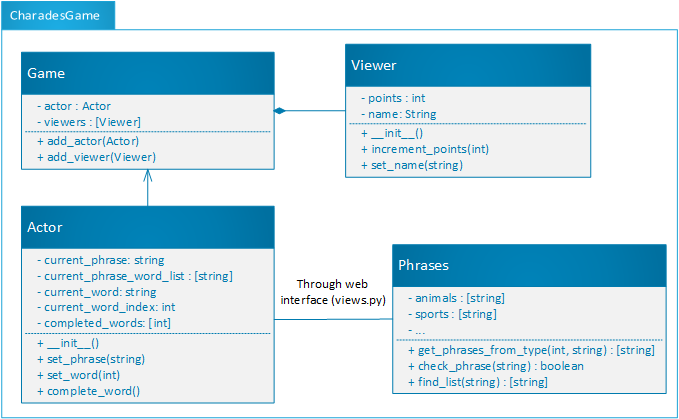
\includegraphics[width=\textwidth]{CharadesGameClass}


\section{Description of Class Diagram}
This is an additional architecture embedded into the Django website. These classes will manage the information that needs to be stored for each player as well as checks to ensure the session has the correct number of players. 

\subsection{Actor}
\subsubsection{Variables}
\begin{itemize}

	\item \textbf{current\_phrase}: Contains the current phrase that the Actor is attempting to act. Type: String.
	
	\item \textbf{current\_phrase\_word\_list}: A list of the words within the phrase. This will be created using the python split() function which separates a string by spaces. This variable will save time having to look up the word each time to display it. Type: string list.

	\item \textbf{current\_word}: Contains the current word in the phrase that is being acted. This is an integer that relates to word. Type: int.
	
	\item \textbf{current\_word\_index}: Holds the current index of the word being acted / guessed. Type: int.
	
	\item \textbf{completed\_words}: A list of integers representing the words that have been completed. A word is completed when it correctly guessed or time has elapsed. Type: int list.
	
\end{itemize}

\subsubsection{Functions}

\begin{itemize}

	\item \textbf{\_\_init\_\_}: Resets the variables to default values.

	\item \textbf{set\_phrase}: updates the phrase variable with a new string.
	
	\item \textbf{set\_word}: updates the word variable with a  new int.
	
	\item \textbf{complete\_word}: adds a word (int) to the completed word list.

\end{itemize}


\subsection{Viewer}
\subsubsection{Variables}

\begin{itemize}
	\item \textbf{points}: The number of points accumulated by the viewer. Type: int.

	\item \textbf{name}: The name of the viewer. Type: String.

\end{itemize}

\subsection{Functions}

\begin{itemize}

	\item \textbf{\_\_init\_\_}: Resets the variables to default values.

	\item \textbf{increment\_points}: increase the points variable by an integer.
	
	\item \textbf{set\_name}: updates the name variable with a String.
	
\end{itemize}

\subsection{Game}
\subsubsection{Variables}
\begin{itemize}
	\item \textbf{actor}: The actor in the game. (There is only one actor per game. Type: Actor
	
	\item \textbf{viewers}: A list of the viewers in the game. Type: Viewer list.
	
\end{itemize}

\subsection{Functions}
\begin{itemize}

	\item \textbf{add\_actor}: Updates the actor variable with a new Actor.
	
	\item \textbf{add\_viewer}: Adds a Viewer to the viewer list variable. There will be a check to ensure the same viewer is not being added again as well as ensure the maximum number of viewers is not exceeded.
	
\end{itemize}

\end{document}